\documentclass[12pt,fleqn]{article}\usepackage{../../common}
\begin{document}
Döndürme (Rotation) - 2

Herhangi Bir Eksen (Vektör) Etrafında Dönüş

Daha öne Rodriguez yöntemi ile yaptığımız döndürme yaklaşımını bir başka
teknikle göstereceğiz. Bulmak istediğimiz $\vec{n}$ etrafında $\theta$ dönüşü
yaptıracak bir matris, yani öyle bir matris $R(\vec{n},\theta)$ arıyoruz ki bu
matrisle $\vec{v}$ vektörünü sağdan çarpınca $\vec{v}'$ elde edilecek ve bu yeni
vektör $\vec{v}$ vektörünün $\vec{n}$ etrafında $\theta$ kadar dönmüş hali
olacak,

$$
v' = v R(n,\theta)
$$

$R(n,\theta)$ matrisini türetmek için önce $v'$ vektörünü $v,n,\theta$ bazında
temsil etmeyi görelim. Ana fikir problemi $n$'ye dik olan düzlem üzerinde
çözmek, ki bu şekilde 3 boyutlu problemi 2 boyutlu bir probleme indirgemiş
oluyoruz. İndirgeme için $v$ vektörünü iki $v_\parallel$ ve $v_\perp$ vektörüne
ayıracağız, öyle ki $v = v_\parallel + v_\perp$. Sonra bu ki vektörü ayrıca
döndüreceğiz ve böylece onların toplamları da dönmüş olacak, yani $v' =
v'_\parallel + v'_\perp$. Buraya kadar gördüklerimiz Rodriguez yaklaşımına
benziyor.

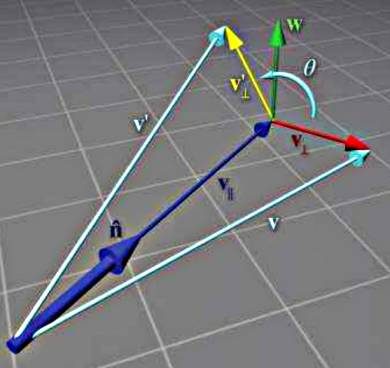
\includegraphics[width=10em]{phy_073_rot_01.jpg}

Tekniğin iyi tarafı $v_\parallel$ vektörü $n$ vektörüne paralel olduğu için $n$
etrafında dönüşten etkilenmez, o zaman sadece $v_\perp$ vektörünü döndürmek
yeterlidir, böylece $v' = v_\parallel + v'_\perp$ hesaplanabilir.

Hesap için şu adımları takip ediyoruz,

\begin{itemize}
   \item $v_\parallel$ vektörü $v$ nin $n$ ye paralel olan şeklidir, ya da
     $v$ vektörünün $n$ üzerinde yansıtılmış halidir [2], bu formülün
     $v_\parallel = (v \cdot n) n$ olduğunu biliyoruz.
   \item $v_\perp$ vektoru $v$ nin $n$ ye dik olan kismidir.
     $v = v_\parallel + v_\perp$ oldugu icin $v_\perp = v - v_\parallel$.
\end{itemize}




Teori

2D düzlemde, A vektörünün $\theta$ açısı kadar döndürülmesinin, $Y =
\cos \theta A + \sin \theta B$ vektörünü verir.

İspat

A ve B'nin 3D uzayında 2D bir düzlemi kapsayan iki dikgen vektör olduğunu
varsayalım. A ve B'yi bu 2D düzlem için baz vektörleri olarak düşünebiliriz. A
ve B tarafından kapsanan düzlemdeki herhangi bir X vektörü, A ve B'nin bir
doğrusal birleşimi olarak ifade edilebilir:

$X = x_A A + x_B B$

Burada, $x_A$ ve $x_B$, X'in A ve B doğrultularındaki bileşenleridir.

A vektörü için, {A, B} bazındaki temsili, A doğrultusundaki bileşenin
1 ve B doğrultusundaki bileşenin 0 olduğu durumdur. Yani, A'yı bu 2D
baz sisteminde "x ekseni" ve B'yi "y ekseni" olarak düşünebiliriz,
burada A'nın "koordinatları" (1, 0) olur.

Şimdi, A vektörünü A ve B'nin kapsadığı düzlem içinde $\theta$ açısı
kadar döndürelim. Ortaya çıkan vektöre Y diyelim. Standart bir 2D
Kartezyen koordinat sisteminde, koordinatları $(x, y)$ olan bir vektör
$\theta$ açısı kadar saat yönünün tersine döndürüldüğünde, yeni
koordinatları $(x', y')$ şu şekilde bulunur:

$x' = x \cos \theta - y \sin \theta$

$y' = x \sin \theta + y \cos \theta$

Bizim durumumuzda, A vektörünün {A, B} bazındaki başlangıç
"koordinatları" $(1, 0)$'dır. A'yı $\theta$ kadar döndürdüğümüzde,
ortaya çıkan Y vektörünün {A, B} bazındaki yeni "koordinatları",
$(y_A, y_B)$, $(x, y) = (1, 0)$ kullanılarak 2D döndürme formülleriyle
bulunabilir:

$y_A = 1 \cdot \cos \theta - 0 \cdot \sin \theta = \cos \theta$

$y_B = 1 \cdot \sin \theta + 0 \cdot \cos \theta = \sin \theta$

Dolayısıyla, döndürülen Y vektörünün {A, B} bazındaki bileşenleri, A
doğrultusunda $\cos \theta$ ve B doğrultusunda $\sin \theta$ olur.

Şimdi Y vektörünü, bu bileşenleri kullanarak baz vektörler A ve B'nin
doğrusal birleşimi olarak yazabiliriz:

$Y = y_A A + y_B B$

$Y = \cos \theta A + \sin \theta B$

Bu, A vektörünün A ve B'nin kapsadığı 2D düzlem içinde $\theta$ açısı
kadar döndürülmesinin $Y = \cos \theta A + \sin \theta B$ vektörünü
verdiğini kanıtlar. Bu, bir 2D Kartezyen düzlemde x eksenindeki $(1,
0)$ vektörünün $\theta$ kadar döndürüldüğünde $(\cos \theta, \sin
\theta)$'ye dönmesiyle benzerdir. A ve B vektörleri, 3D uzayında bu 2D
dönüşüm için eksenleri sağlar.

Kaynaklar

[1] Dunn, {\em 3D Math Primer for Graphics and Game Development}

[2] Bayramlı, {\em Lineer Cebir - Giriş}

\end{document}
